\begin{problem}[James_SUVAT]
{If a body is undergoing constant acceleration, then its acceleration can be defined as $a~=~\frac{\textrm{Change in speed}}{\textrm{Time taken to change speed}}~=~\frac{v - u}{t}$ where $u$ is the initial speed and $v$ the final speed of the body in the time period $t$.
\begin{enumerate}
	\item In terms of $u$, $v$ and $t$ and by using the definition of average speed; what distance, $s$, does the body travel in a time $t$?
	\item Using the equation $a = \frac{v - u}{t}$ and the equation derived in (a) for $s$:
	\begin{enumerate}
		\item Write an equation for $s$ that does not involve $v$,
		\item Write an equation for $s$ that does not involve $u$,
		\item Write an equation for $s$ that does not involve $t$.
	\end{enumerate}
	Bonus: The two equations in (b)i and (b)ii can be found graphically from a speed-time graph. If at $t = 0$ the body has speed $u$ and at time $t$ has speed $v$, plot a graph showing this motion and explain graphically the origins of the equations for $s$.
\end{enumerate}
}
{\textit{Created for the Rutherford School Physics Project by JS.}}
{This question derives the five SUVAT equations from the simplest two equations that can be justified by prior knowledge.
\begin{enumerate}
	\item If a body is moving with constant acceleration, then its average speed is simply $\bar{v} = \frac{u+v}{2}$. The distance covered is then the average speed times the time: $s = \bar{v}t = \left(\frac{u+v}{2}\right)t$.
	\item Part b) derives the other three SUVAT equations:
	\begin{enumerate}
		\item We can use the equation $s = \left(\frac{u + v}{2}\right)t$ and substitute $v = u + at$ to get the equation $s = \left(\frac{2u + at}{2}\right)t$. Rearrange to get $s = ut + \frac{1}{2}at^{2}$.
		\item Rearrange $v = u + at$ to get $u = v - at$, then substitute this value of $u$ into $s = \left(\frac{u + v}{2}\right)t$ to get $s = \left(\frac{2v - at}{2}\right)t$. Rearrange to find the solution, $s = vt - \frac{1}{2}at^{2}$.
		\item Rearrange $v = u + at$ in terms of $t$ to get $t = \frac{v - u}{a}$. Substitute this value into $s = \left(\frac{u + v}{2}\right)t$ to get $s = \frac{(v + u)(v - u)}{2a} = \frac{v^{2} - u^{2}}{2a}$.
	\end{enumerate}
	Bonus: The area under a speed-time graph as shown in Figure \ref{fig:Kinematics_SUVAT_graph} is equal to the distance travelled, $s$, and the gradient of the line is equal to the acceleration, $a$. It is therefore possible to find an expression for $s$ by calculating the area under the graph, and we can do this in two different ways: (1) by adding the areas of rectangle A and triangle B, or (2) by subtracting the area of triangle C from the area of the large overall rectangle. The areas of triangles B and C are equal; they both have base = $t$, and height = gradient $\times~t = at$. Therefore, the area of each triangle $= \frac{1}{2}(t)(at) = \frac{1}{2}at^{2}$. The area of rectangle A = base $\times$ height $= ut$ and the area of the large overall rectangle $= vt$.

Method (1) of calculating the area gives $s = ut + \frac{1}{2}at^{2}$, which is the result from question b)i. Method (2) gives $s = vt - \frac{1}{2}at^{2}$, as shown in question b)ii.
\begin{figure}[h]
\centering
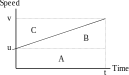
\includegraphics[width=0.4\textwidth]{Kinematics_SUVAT_graph}
\caption{}
\label{fig:Kinematics_SUVAT_graph}
\end{figure}	

N.B. It is also possible to demonstrate the relationship $v = u + at$ from this graph; we can easily see that the difference in height between $v$ and $u$ is equal to the gradient of the line, $a$, multiplied by the time taken, $t$.
\end{enumerate}
 }
\end{problem}